\PassOptionsToPackage{unicode=true}{hyperref} % options for packages loaded elsewhere
\PassOptionsToPackage{hyphens}{url}
%
\documentclass[]{article}
\usepackage{lmodern}
\usepackage{amssymb,amsmath}
\usepackage{ifxetex,ifluatex}
\usepackage{fixltx2e} % provides \textsubscript
\ifnum 0\ifxetex 1\fi\ifluatex 1\fi=0 % if pdftex
  \usepackage[T1]{fontenc}
  \usepackage[utf8]{inputenc}
  \usepackage{textcomp} % provides euro and other symbols
\else % if luatex or xelatex
  \usepackage{unicode-math}
  \defaultfontfeatures{Ligatures=TeX,Scale=MatchLowercase}
\fi
% use upquote if available, for straight quotes in verbatim environments
\IfFileExists{upquote.sty}{\usepackage{upquote}}{}
% use microtype if available
\IfFileExists{microtype.sty}{%
\usepackage[]{microtype}
\UseMicrotypeSet[protrusion]{basicmath} % disable protrusion for tt fonts
}{}
\IfFileExists{parskip.sty}{%
\usepackage{parskip}
}{% else
\setlength{\parindent}{0pt}
\setlength{\parskip}{6pt plus 2pt minus 1pt}
}
\usepackage{hyperref}
\hypersetup{
            pdftitle={Compulsory Exercise 2: Group 37},
            pdfauthor={Anders Bendiksen and Helge Bergo},
            pdfborder={0 0 0},
            breaklinks=true}
\urlstyle{same}  % don't use monospace font for urls
\usepackage[margin=1in]{geometry}
\usepackage{color}
\usepackage{fancyvrb}
\newcommand{\VerbBar}{|}
\newcommand{\VERB}{\Verb[commandchars=\\\{\}]}
\DefineVerbatimEnvironment{Highlighting}{Verbatim}{commandchars=\\\{\}}
% Add ',fontsize=\small' for more characters per line
\usepackage{framed}
\definecolor{shadecolor}{RGB}{248,248,248}
\newenvironment{Shaded}{\begin{snugshade}}{\end{snugshade}}
\newcommand{\AlertTok}[1]{\textcolor[rgb]{0.94,0.16,0.16}{#1}}
\newcommand{\AnnotationTok}[1]{\textcolor[rgb]{0.56,0.35,0.01}{\textbf{\textit{#1}}}}
\newcommand{\AttributeTok}[1]{\textcolor[rgb]{0.77,0.63,0.00}{#1}}
\newcommand{\BaseNTok}[1]{\textcolor[rgb]{0.00,0.00,0.81}{#1}}
\newcommand{\BuiltInTok}[1]{#1}
\newcommand{\CharTok}[1]{\textcolor[rgb]{0.31,0.60,0.02}{#1}}
\newcommand{\CommentTok}[1]{\textcolor[rgb]{0.56,0.35,0.01}{\textit{#1}}}
\newcommand{\CommentVarTok}[1]{\textcolor[rgb]{0.56,0.35,0.01}{\textbf{\textit{#1}}}}
\newcommand{\ConstantTok}[1]{\textcolor[rgb]{0.00,0.00,0.00}{#1}}
\newcommand{\ControlFlowTok}[1]{\textcolor[rgb]{0.13,0.29,0.53}{\textbf{#1}}}
\newcommand{\DataTypeTok}[1]{\textcolor[rgb]{0.13,0.29,0.53}{#1}}
\newcommand{\DecValTok}[1]{\textcolor[rgb]{0.00,0.00,0.81}{#1}}
\newcommand{\DocumentationTok}[1]{\textcolor[rgb]{0.56,0.35,0.01}{\textbf{\textit{#1}}}}
\newcommand{\ErrorTok}[1]{\textcolor[rgb]{0.64,0.00,0.00}{\textbf{#1}}}
\newcommand{\ExtensionTok}[1]{#1}
\newcommand{\FloatTok}[1]{\textcolor[rgb]{0.00,0.00,0.81}{#1}}
\newcommand{\FunctionTok}[1]{\textcolor[rgb]{0.00,0.00,0.00}{#1}}
\newcommand{\ImportTok}[1]{#1}
\newcommand{\InformationTok}[1]{\textcolor[rgb]{0.56,0.35,0.01}{\textbf{\textit{#1}}}}
\newcommand{\KeywordTok}[1]{\textcolor[rgb]{0.13,0.29,0.53}{\textbf{#1}}}
\newcommand{\NormalTok}[1]{#1}
\newcommand{\OperatorTok}[1]{\textcolor[rgb]{0.81,0.36,0.00}{\textbf{#1}}}
\newcommand{\OtherTok}[1]{\textcolor[rgb]{0.56,0.35,0.01}{#1}}
\newcommand{\PreprocessorTok}[1]{\textcolor[rgb]{0.56,0.35,0.01}{\textit{#1}}}
\newcommand{\RegionMarkerTok}[1]{#1}
\newcommand{\SpecialCharTok}[1]{\textcolor[rgb]{0.00,0.00,0.00}{#1}}
\newcommand{\SpecialStringTok}[1]{\textcolor[rgb]{0.31,0.60,0.02}{#1}}
\newcommand{\StringTok}[1]{\textcolor[rgb]{0.31,0.60,0.02}{#1}}
\newcommand{\VariableTok}[1]{\textcolor[rgb]{0.00,0.00,0.00}{#1}}
\newcommand{\VerbatimStringTok}[1]{\textcolor[rgb]{0.31,0.60,0.02}{#1}}
\newcommand{\WarningTok}[1]{\textcolor[rgb]{0.56,0.35,0.01}{\textbf{\textit{#1}}}}
\usepackage{graphicx,grffile}
\makeatletter
\def\maxwidth{\ifdim\Gin@nat@width>\linewidth\linewidth\else\Gin@nat@width\fi}
\def\maxheight{\ifdim\Gin@nat@height>\textheight\textheight\else\Gin@nat@height\fi}
\makeatother
% Scale images if necessary, so that they will not overflow the page
% margins by default, and it is still possible to overwrite the defaults
% using explicit options in \includegraphics[width, height, ...]{}
\setkeys{Gin}{width=\maxwidth,height=\maxheight,keepaspectratio}
\setlength{\emergencystretch}{3em}  % prevent overfull lines
\providecommand{\tightlist}{%
  \setlength{\itemsep}{0pt}\setlength{\parskip}{0pt}}
\setcounter{secnumdepth}{0}
% Redefines (sub)paragraphs to behave more like sections
\ifx\paragraph\undefined\else
\let\oldparagraph\paragraph
\renewcommand{\paragraph}[1]{\oldparagraph{#1}\mbox{}}
\fi
\ifx\subparagraph\undefined\else
\let\oldsubparagraph\subparagraph
\renewcommand{\subparagraph}[1]{\oldsubparagraph{#1}\mbox{}}
\fi

% set default figure placement to htbp
\makeatletter
\def\fps@figure{htbp}
\makeatother

\usepackage{etoolbox}
\makeatletter
\providecommand{\subtitle}[1]{% add subtitle to \maketitle
  \apptocmd{\@title}{\par {\large #1 \par}}{}{}
}
\makeatother

\title{Compulsory Exercise 2: Group 37}
\providecommand{\subtitle}[1]{}
\subtitle{TMA4268 Statistical Learning V2019}
\author{Anders Bendiksen and Helge Bergo}
\date{02 April, 2020}

\begin{document}
\maketitle

\hypertarget{problem-1-10p}{%
\section{Problem 1 (10p)}\label{problem-1-10p}}

\hypertarget{a-ridge-regression-2p}{%
\subsection{a) Ridge Regression (2p)}\label{a-ridge-regression-2p}}

Show that the ridge regression estimator is
\(\hat\beta_{Ridge} = (X^T X + \lambda I)^{-1} X^T y\).

\hypertarget{b-2p}{%
\subsection{b) (2p)}\label{b-2p}}

Find the expected value and the variance-covariance matrix of
\(\hat\beta_{Ridge}\) (1P each).

\hypertarget{c-2p---multiple-choice}{%
\subsection{c) (2P) - Multiple choice}\label{c-2p---multiple-choice}}

\begin{enumerate}
\def\labelenumi{(\roman{enumi})}
\tightlist
\item
  TRUE
\item
  FALSE
\item
  FALSE
\item
  TRUE
\end{enumerate}

\hypertarget{d-forward-selection}{%
\subsection{d) Forward Selection}\label{d-forward-selection}}

\begin{Shaded}
\begin{Highlighting}[]
\KeywordTok{library}\NormalTok{(ISLR)}
\KeywordTok{set.seed}\NormalTok{(}\DecValTok{1}\NormalTok{)}
\NormalTok{train.ind =}\StringTok{ }\KeywordTok{sample}\NormalTok{(}\DecValTok{1}\OperatorTok{:}\KeywordTok{nrow}\NormalTok{(College), }\FloatTok{0.5}\OperatorTok{*}\KeywordTok{nrow}\NormalTok{(College))}
\NormalTok{college.train =}\StringTok{ }\NormalTok{College[train.ind,]}
\NormalTok{college.test =}\StringTok{ }\NormalTok{College[}\OperatorTok{-}\NormalTok{train.ind,]}
\end{Highlighting}
\end{Shaded}

After dividing the data into a training and test set, the
\texttt{regsubsets} function was used to create a forward selection
model on the data, from the \texttt{leaps}-library.

\begin{Shaded}
\begin{Highlighting}[]
\KeywordTok{library}\NormalTok{(leaps)}
\NormalTok{regfit.fwd =}\StringTok{ }\KeywordTok{regsubsets}\NormalTok{(Outstate}\OperatorTok{~}\NormalTok{.,}\DataTypeTok{data=}\NormalTok{college.train,}\DataTypeTok{method=}\StringTok{"forward"}\NormalTok{, }\DataTypeTok{nvmax =} \DecValTok{18}\NormalTok{)}
\NormalTok{reg.summary =}\StringTok{ }\KeywordTok{summary}\NormalTok{(regfit.fwd)}
\end{Highlighting}
\end{Shaded}

To decide on which model is best, the number of variables used in the
selection was plotted against \texttt{RSS}, \texttt{Cp}, \texttt{BIC}
and \texttt{adjusted\ R\$\^{}2\$}.

\begin{Shaded}
\begin{Highlighting}[]
\KeywordTok{par}\NormalTok{(}\DataTypeTok{mfrow=}\KeywordTok{c}\NormalTok{(}\DecValTok{2}\NormalTok{,}\DecValTok{2}\NormalTok{))}
\KeywordTok{plot}\NormalTok{(reg.summary}\OperatorTok{$}\NormalTok{rss,}\DataTypeTok{xlab=}\StringTok{"Number of variables"}\NormalTok{,}\DataTypeTok{ylab=}\StringTok{"RSS"}\NormalTok{,}\DataTypeTok{type=}\StringTok{"b"}\NormalTok{)}

\KeywordTok{plot}\NormalTok{(reg.summary}\OperatorTok{$}\NormalTok{adjr2,}\DataTypeTok{xlab=}\StringTok{"Number of variables"}\NormalTok{,}\DataTypeTok{ylab=}\StringTok{"Adjusted Rsq"}\NormalTok{,}\DataTypeTok{type=}\StringTok{"b"}\NormalTok{)}
\NormalTok{max.adjr2 =}\StringTok{ }\KeywordTok{which.max}\NormalTok{(reg.summary}\OperatorTok{$}\NormalTok{adjr2)}
\KeywordTok{points}\NormalTok{(max.adjr2,reg.summary}\OperatorTok{$}\NormalTok{adjr2[max.adjr2], }\DataTypeTok{col=}\StringTok{"black"}\NormalTok{,}\DataTypeTok{cex=}\DecValTok{2}\NormalTok{,}\DataTypeTok{pch=}\DecValTok{20}\NormalTok{)}

\KeywordTok{plot}\NormalTok{(reg.summary}\OperatorTok{$}\NormalTok{cp,}\DataTypeTok{xlab=}\StringTok{"Number of variables"}\NormalTok{,}\DataTypeTok{ylab=}\StringTok{"Cp"}\NormalTok{,}\DataTypeTok{type=}\StringTok{"b"}\NormalTok{)}
\NormalTok{min.cp =}\StringTok{ }\KeywordTok{which.min}\NormalTok{(reg.summary}\OperatorTok{$}\NormalTok{cp)}
\KeywordTok{points}\NormalTok{(min.cp,reg.summary}\OperatorTok{$}\NormalTok{cp[min.cp], }\DataTypeTok{col=}\StringTok{"black"}\NormalTok{,}\DataTypeTok{cex=}\DecValTok{2}\NormalTok{,}\DataTypeTok{pch=}\DecValTok{20}\NormalTok{)}

\KeywordTok{plot}\NormalTok{(reg.summary}\OperatorTok{$}\NormalTok{bic,}\DataTypeTok{xlab=}\StringTok{"Number of variables"}\NormalTok{,}\DataTypeTok{ylab=}\StringTok{"BIC"}\NormalTok{,}\DataTypeTok{type=}\StringTok{"b"}\NormalTok{)}
\NormalTok{min.bic =}\StringTok{ }\KeywordTok{which.min}\NormalTok{(reg.summary}\OperatorTok{$}\NormalTok{bic)}
\KeywordTok{points}\NormalTok{(min.bic,reg.summary}\OperatorTok{$}\NormalTok{bic[min.bic], }\DataTypeTok{col=}\StringTok{"black"}\NormalTok{,}\DataTypeTok{cex=}\DecValTok{2}\NormalTok{,}\DataTypeTok{pch=}\DecValTok{20}\NormalTok{)}
\end{Highlighting}
\end{Shaded}

\begin{center}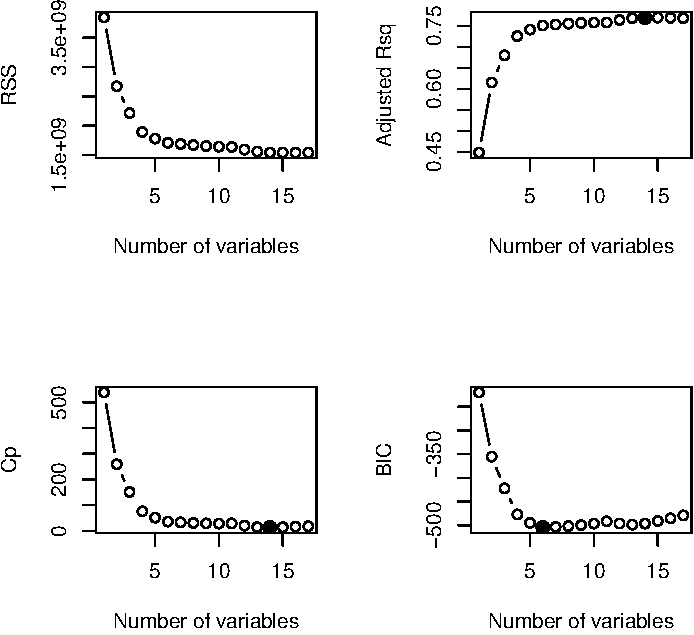
\includegraphics{Compulsory2_Group37_StatLearn_files/figure-latex/p2d3-1} \end{center}

The maximum \texttt{adjusted} \(R^2\) is the one with 14 variables, with
a value of 0.7706887, shown as a filled dot in the upper right plot.
This is also the same number of variables as for the lowest Cp. However,
all the plots are pretty flat after around 6 or 7 variables used, and it
seems like using only 6 variables still gives a good \texttt{adjusted}
\(R^2\) value of 0.7516133, without the increased complexity of adding 7
more variables. The model is then:

\begin{Shaded}
\begin{Highlighting}[]
\KeywordTok{coef}\NormalTok{(regfit.fwd,}\DecValTok{6}\NormalTok{)}
\end{Highlighting}
\end{Shaded}

\begin{verbatim}
##   (Intercept)    PrivateYes    Room.Board      Terminal   perc.alumni 
## -4726.8810613  2717.7019276     1.1032433    36.9990286    59.0863753 
##        Expend     Grad.Rate 
##     0.1930814    33.8303314
\end{verbatim}

For the MSE, the following code calculates the MSE for all the
variables.

\begin{Shaded}
\begin{Highlighting}[]
\NormalTok{val.errors =}\StringTok{ }\KeywordTok{rep}\NormalTok{(}\OtherTok{NA}\NormalTok{,}\DecValTok{17}\NormalTok{)}
\NormalTok{x.test =}\StringTok{ }\KeywordTok{model.matrix}\NormalTok{(Outstate}\OperatorTok{~}\NormalTok{.,}\DataTypeTok{data=}\NormalTok{college.test) }\CommentTok{# notice the -index!}
\ControlFlowTok{for}\NormalTok{ (i }\ControlFlowTok{in} \DecValTok{1}\OperatorTok{:}\DecValTok{17}\NormalTok{) \{}
\NormalTok{    coefi =}\StringTok{ }\KeywordTok{coef}\NormalTok{(regfit.fwd,}\DataTypeTok{id=}\NormalTok{i)}
\NormalTok{    pred =}\StringTok{ }\NormalTok{x.test[,}\KeywordTok{names}\NormalTok{(coefi)]}\OperatorTok\NormalTok{coefi}
\NormalTok{    val.errors[i] =}\StringTok{ }\KeywordTok{mean}\NormalTok{((college.test}\OperatorTok{$}\NormalTok{Outstate}\OperatorTok{-}\NormalTok{pred)}\OperatorTok{^}\DecValTok{2}\NormalTok{)}
\NormalTok{\}}

\CommentTok{# plot(sqrt(val.errors),xlab="Number of variables", ylab="Root MSE",ylim=c(1500,5000) ,pch=19,type="b")}
\CommentTok{# points(sqrt(regfit.fwd$rss[-1]/180),col="blue",pch=19,type="b")}
\CommentTok{# legend("topright",legend=c("Training","Validation"),col=c("black","blue"),pch=19)}
\end{Highlighting}
\end{Shaded}

The MSE of the model with 6 variables is then:

\begin{Shaded}
\begin{Highlighting}[]
\NormalTok{val.errors[}\DecValTok{6}\NormalTok{]}
\end{Highlighting}
\end{Shaded}

\begin{verbatim}
## [1] 3844857
\end{verbatim}

\hypertarget{e-2p}{%
\subsection{e) (2p)}\label{e-2p}}

Using the Lasso method from the \texttt{glmnet}-library, a new model was
selected.

To select the tuning parameter \(\lambda\), cross-validation was
performed, and the \(\lambda\) giving the lowest MSE was selected.

\begin{Shaded}
\begin{Highlighting}[]
\NormalTok{cv.out =}\StringTok{ }\KeywordTok{cv.glmnet}\NormalTok{(x.train,y.train, }\DataTypeTok{alpha =} \DecValTok{1}\NormalTok{)}
\KeywordTok{plot}\NormalTok{(cv.out)}
\end{Highlighting}
\end{Shaded}

\begin{center}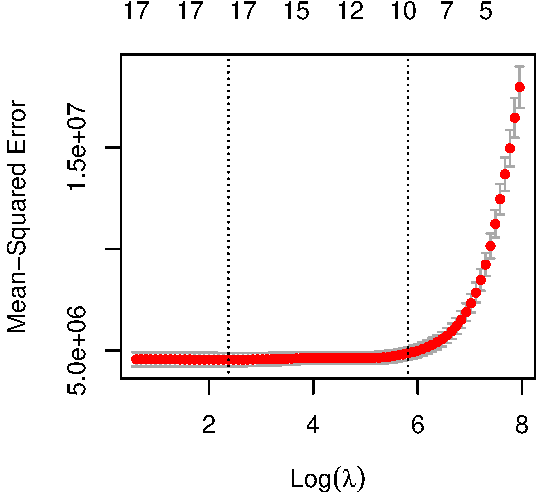
\includegraphics{Compulsory2_Group37_StatLearn_files/figure-latex/unnamed-chunk-10-1} \end{center}

\begin{Shaded}
\begin{Highlighting}[]
\NormalTok{best.lambda =}\StringTok{ }\NormalTok{cv.out}\OperatorTok{$}\NormalTok{lambda.min}
\NormalTok{best.lambda}
\end{Highlighting}
\end{Shaded}

\begin{verbatim}
## [1] 10.7207
\end{verbatim}

This was used on the test set, to get the MSE for the

\begin{Shaded}
\begin{Highlighting}[]
\NormalTok{lasso.pred =}\StringTok{ }\KeywordTok{predict}\NormalTok{(lasso.model,}\DataTypeTok{s=}\NormalTok{best.lambda ,}\DataTypeTok{newx=}\NormalTok{x.test)}
\NormalTok{MSE =}\StringTok{ }\KeywordTok{mean}\NormalTok{((lasso.pred}\OperatorTok{-}\NormalTok{y.test)}\OperatorTok{^}\DecValTok{2}\NormalTok{)}
\NormalTok{MSE}
\end{Highlighting}
\end{Shaded}

\begin{verbatim}
## [1] 3688061
\end{verbatim}

Finally, the coefficients of the model are shown here:

\begin{Shaded}
\begin{Highlighting}[]
\NormalTok{lasso.coef =}\StringTok{ }\KeywordTok{predict}\NormalTok{(cv.out,}\DataTypeTok{type=}\StringTok{"coefficients"}\NormalTok{,}\DataTypeTok{s=}\NormalTok{best.lambda)[}\DecValTok{1}\OperatorTok{:}\DecValTok{18}\NormalTok{,]}
\NormalTok{lasso.coef}
\end{Highlighting}
\end{Shaded}

\begin{verbatim}
##   (Intercept)    PrivateYes          Apps        Accept        Enroll 
## -1.172140e+03  2.230467e+03 -2.825215e-01  6.615811e-01 -3.778631e-01 
##     Top10perc     Top25perc   F.Undergrad   P.Undergrad    Room.Board 
##  4.589180e+01 -1.485674e+01 -5.800132e-02 -5.713770e-02  1.088115e+00 
##         Books      Personal           PhD      Terminal     S.F.Ratio 
## -9.185125e-01 -3.005419e-01  4.013410e+00  2.996744e+01 -6.936391e+01 
##   perc.alumni        Expend     Grad.Rate 
##  4.686967e+01  1.480013e-01  2.431539e+01
\end{verbatim}

\hypertarget{problem-2-9p}{%
\section{Problem 2 (9p)}\label{problem-2-9p}}

\hypertarget{a-2p---multiple-choice}{%
\subsection{a) (2p) - Multiple choice}\label{a-2p---multiple-choice}}

Which of the following statements are true, which false?

\begin{enumerate}
\def\labelenumi{(\roman{enumi})}
\item
  A regression spline of order 3 with 4 knots has 8 basis functions.
\item
  A regression spline with polynomials of degree \(M-1\) has continuous
  derivatives up to order \(M-2,\) but not at the knots.
\item
  A natural cubic spline is linear beyond the boundary knots.
\item
  A smoothing spline is (a shrunken version of) a natural cubic spline
  with knots at the values of all data points \(x_i\) for
  \(i=1,\ldots ,n\).
\item
\item
\item
\item
\end{enumerate}

\hypertarget{b-2p-1}{%
\subsection{b) (2p)}\label{b-2p-1}}

Write down the basis functions for a cubic spline with knots at the
quartiles \(q_1, q_2, q_3\) of variable \(X\).

\hypertarget{c-2p}{%
\subsection{c) (2p)}\label{c-2p}}

\begin{center}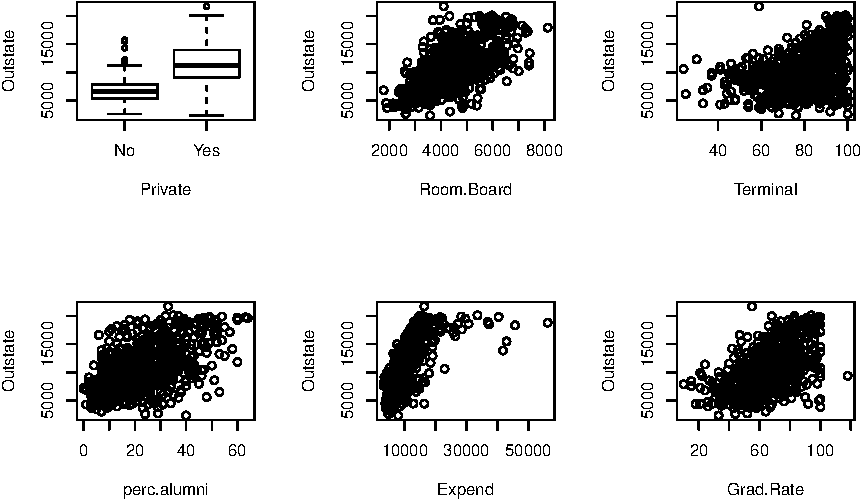
\includegraphics{Compulsory2_Group37_StatLearn_files/figure-latex/2c3-1} \end{center}

From these plots, it seems like \texttt{Room.board},
\texttt{perc.alumni} and \texttt{Grad.Rate} all have quite linear
relationships with \texttt{Outstate}, while both \texttt{Terminal} and
\texttt{Expend} seem to follow a non-linear relationship.

\hypertarget{d-3p}{%
\subsection{d) (3P)}\label{d-3p}}

\begin{enumerate}
\def\labelenumi{(\roman{enumi})}
\tightlist
\item
  Fit polynomial regression models for \texttt{Outstate} with
  \texttt{Terminal} as the only covariate for a range of polynomial
  degrees (\(d = 1,\ldots,10\)) and plot the results. Use the training
  data (\texttt{college.train}) for this task.
\end{enumerate}

\begin{Shaded}
\begin{Highlighting}[]
\NormalTok{cols =}\StringTok{ }\KeywordTok{rainbow}\NormalTok{(}\DecValTok{10}\NormalTok{)}
\NormalTok{deg =}\StringTok{ }\DecValTok{1}\OperatorTok{:}\DecValTok{10}
\NormalTok{polyfunc =}\StringTok{ }\ControlFlowTok{function}\NormalTok{(d) \{}
\NormalTok{  model =}\StringTok{ }\KeywordTok{lm}\NormalTok{(Outstate }\OperatorTok{~}\StringTok{ }\KeywordTok{poly}\NormalTok{(Terminal,d), }\DataTypeTok{data=}\NormalTok{college.train)}
  \KeywordTok{lines}\NormalTok{(}\KeywordTok{cbind}\NormalTok{(college.train}\OperatorTok{$}\NormalTok{Terminal, model}\OperatorTok{$}\NormalTok{fit)[}\KeywordTok{order}\NormalTok{(college.train}\OperatorTok{$}\NormalTok{Terminal),],}\DataTypeTok{col=}\NormalTok{cols[d])}
\NormalTok{  pred =}\StringTok{ }\KeywordTok{predict}\NormalTok{(model, college.train)}
  \KeywordTok{mean}\NormalTok{((pred }\OperatorTok{-}\StringTok{ }\NormalTok{college.train}\OperatorTok{$}\NormalTok{Outstate)}\OperatorTok{^}\DecValTok{2}\NormalTok{)}
\NormalTok{\}}
\KeywordTok{plot}\NormalTok{(college.train}\OperatorTok{$}\NormalTok{Terminal, college.train}\OperatorTok{$}\NormalTok{Outstate, }\DataTypeTok{col =} \StringTok{"gray"}\NormalTok{, }\DataTypeTok{pch=}\DecValTok{19}\NormalTok{, }
     \DataTypeTok{cex =} \FloatTok{0.5}\NormalTok{, }\DataTypeTok{xlab =} \StringTok{"Terminal"}\NormalTok{, }\DataTypeTok{ylab =} \StringTok{"Outstate"}\NormalTok{)}
\NormalTok{MSE =}\StringTok{ }\KeywordTok{sapply}\NormalTok{(deg, polyfunc)}
\KeywordTok{legend}\NormalTok{(}\StringTok{"topleft"}\NormalTok{,}\DataTypeTok{legend =} \KeywordTok{paste}\NormalTok{(}\StringTok{"degree = "}\NormalTok{,deg), }\DataTypeTok{col =}\NormalTok{ cols, }\DataTypeTok{cex =} \FloatTok{0.4}\NormalTok{)}
\end{Highlighting}
\end{Shaded}

\begin{center}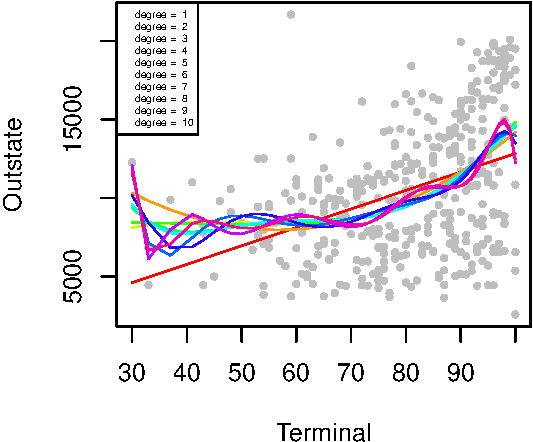
\includegraphics{Compulsory2_Group37_StatLearn_files/figure-latex/2di-1} \end{center}

\begin{enumerate}
\def\labelenumi{(\roman{enumi})}
\setcounter{enumi}{1}
\tightlist
\item
  Still for the training data, choose a suitable smoothing spline model
  to predict \texttt{Outstate} as a function of \texttt{Expend} (again
  as the only covariate) and plot the fitted function into the
  scatterplot of \texttt{Outstate} against \texttt{Expend}. How did you
  choose the degrees of freedom?
\end{enumerate}

\begin{Shaded}
\begin{Highlighting}[]
\KeywordTok{library}\NormalTok{(splines)}
\KeywordTok{attach}\NormalTok{(college.train)}
\NormalTok{expend.range =}\StringTok{ }\KeywordTok{range}\NormalTok{(Expend)}
\NormalTok{expend.grid =}\StringTok{ }\KeywordTok{seq}\NormalTok{(}\DataTypeTok{from=}\NormalTok{expend.range[}\DecValTok{1}\NormalTok{],}\DataTypeTok{to=}\NormalTok{expend.range[}\DecValTok{2}\NormalTok{])}

\KeywordTok{plot}\NormalTok{(Expend, Outstate, }\DataTypeTok{col =} \StringTok{"darkgrey"}\NormalTok{, }\DataTypeTok{pch=}\DecValTok{19}\NormalTok{, }\DataTypeTok{cex =} \FloatTok{0.5}\NormalTok{)}
\NormalTok{fit.smoothspline =}\StringTok{ }\KeywordTok{smooth.spline}\NormalTok{(Expend,Outstate,}\DataTypeTok{cv=}\OtherTok{TRUE}\NormalTok{)}
\KeywordTok{lines}\NormalTok{(fit.smoothspline)}
\end{Highlighting}
\end{Shaded}

\begin{center}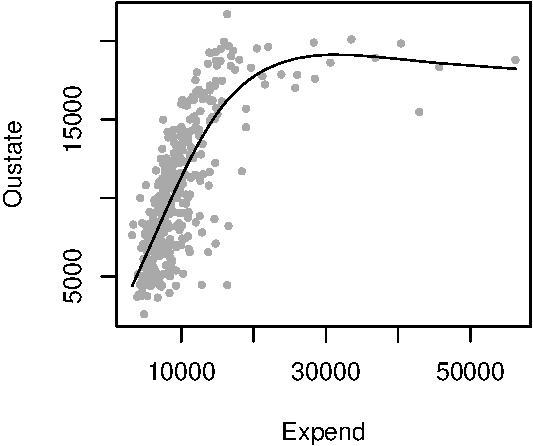
\includegraphics{Compulsory2_Group37_StatLearn_files/figure-latex/2dii-1} \end{center}

\begin{Shaded}
\begin{Highlighting}[]
\CommentTok{# legend("bottomright",legend=paste("DF =",round(fit.smoothspline$df,2)),cex=.8)}
\end{Highlighting}
\end{Shaded}

The degrees of freedom was chosen using cross-validation, and the result
was 4.661.

\begin{enumerate}
\def\labelenumi{(\roman{enumi})}
\setcounter{enumi}{2}
\tightlist
\item
  Report the corresponding training MSE for (i) and (ii). Did you expect
  that?
\end{enumerate}

\begin{Shaded}
\begin{Highlighting}[]
\NormalTok{MSE.smoothspline.train =}\StringTok{ }\KeywordTok{mean}\NormalTok{((}\KeywordTok{predict}\NormalTok{(fit.smoothspline, college.train}\OperatorTok{$}\NormalTok{Expend)}\OperatorTok{$}\NormalTok{y }\OperatorTok{-}\StringTok{ }
\StringTok{                                 }\NormalTok{college.train}\OperatorTok{$}\NormalTok{Outstate)}\OperatorTok{^}\DecValTok{2}\NormalTok{)}
\NormalTok{MSE.smoothspline.train}
\end{Highlighting}
\end{Shaded}

\begin{verbatim}
## [1] 6871281
\end{verbatim}

\begin{Shaded}
\begin{Highlighting}[]
\CommentTok{# MSE.smoothspline.test = mean((predict(fit.smoothspline, college.test$Expend)$y - }
                                \CommentTok{# college.test$Outstate)^2)}
\CommentTok{# MSE.smoothspline.test}
\NormalTok{MSE}
\end{Highlighting}
\end{Shaded}

\begin{verbatim}
##  [1] 15075161 14330586 14249448 14247330 14231485 14230392 14153207 14097911
##  [9] 13841526 13822205
\end{verbatim}

The MSE for the polynomial regression is much higher than the MSE for
the smoothing splines, but this makes a lot of sense when looking at the
initial plots from 2.c). For the \texttt{Expend} variable, it seems like
the data have a clearer trend than for the \texttt{Terminal} variable,
and therefore the MSE is much lower.

\hypertarget{problem-3-9p}{%
\section{Problem 3 (9p)}\label{problem-3-9p}}

\hypertarget{a-2p---multiple-choice-1}{%
\subsection{a) (2P) - Multiple choice}\label{a-2p---multiple-choice-1}}

Which of the following statements are true, which false?

\begin{enumerate}
\def\labelenumi{(\roman{enumi})}
\tightlist
\item
  Regression trees cannot handle categorical predictors.
\item
  Regression and classification trees are easy to interpret.
\item
  The random forest approaches improves bagging, because it reduces the
  variance of the predictor function by decorrelating the trees.
\item
  The number of trees \(B\) in bagging and random forests is a tuning
  parameter.
\end{enumerate}

\hypertarget{b-4p}{%
\subsection{b) (4P)}\label{b-4p}}

Select one method from Module 8 (tree-based methods) in order to build a
good model to predict \texttt{Outstate} in the \texttt{College} dataset
that we used in problems 1 and 2. Explain your choice (pros/cons?) and
how you chose the tuning parameter(s). Train the model using the
training data and report the MSE for the test data.

\hypertarget{c-2p-1}{%
\subsection{c) (2p)}\label{c-2p-1}}

Compare the results (tests MSEs) among all the methods you used in
Problems 1-3. Which method perform best in terms of prediction error?
Which method would you choose if the aim is to develop an interpretable
model?

\hypertarget{problem-4-12p}{%
\section{Problem 4 (12P)}\label{problem-4-12p}}

\hypertarget{a-2p---multiple-choice-2}{%
\subsection{a) (2P) - Multiple choice}\label{a-2p---multiple-choice-2}}

\begin{enumerate}
\def\labelenumi{(\roman{enumi})}
\tightlist
\item
  TRUE
\item
  TRUE
\item
  TRUE
\item
  TRUE
\end{enumerate}

\hypertarget{b-4p-1}{%
\subsection{b) (4P)}\label{b-4p-1}}

First, we convert the variables to factors, and fit a support vector
classifier using the \texttt{e1071} package and the
\texttt{svm}function, and cross validation to find the best cost
parameter.

\begin{Shaded}
\begin{Highlighting}[]
\NormalTok{d.train}\OperatorTok{$}\NormalTok{diabetes <-}\StringTok{ }\KeywordTok{as.factor}\NormalTok{(d.train}\OperatorTok{$}\NormalTok{diabetes)}
\NormalTok{d.test}\OperatorTok{$}\NormalTok{diabetes <-}\StringTok{ }\KeywordTok{as.factor}\NormalTok{(d.test}\OperatorTok{$}\NormalTok{diabetes)}
\KeywordTok{library}\NormalTok{(e1071)}
\KeywordTok{set.seed}\NormalTok{(}\DecValTok{1}\NormalTok{)}

\NormalTok{svm.linear =}\StringTok{ }\KeywordTok{tune}\NormalTok{(svm,diabetes}\OperatorTok{~}\NormalTok{.,}\DataTypeTok{data=}\NormalTok{d.train,}\DataTypeTok{kernel=}\StringTok{"linear"}\NormalTok{, }
                  \DataTypeTok{ranges =} \KeywordTok{list}\NormalTok{(}\DataTypeTok{cost=}\KeywordTok{c}\NormalTok{(}\FloatTok{0.001}\NormalTok{,}\FloatTok{0.01}\NormalTok{,}\FloatTok{0.1}\NormalTok{,}\DecValTok{1}\NormalTok{,}\DecValTok{5}\NormalTok{,}\DecValTok{10}\NormalTok{,}\DecValTok{100}\NormalTok{)))}
\NormalTok{svm.linear.pred  =}\StringTok{ }\KeywordTok{predict}\NormalTok{(svm.linear}\OperatorTok{$}\NormalTok{best.model,d.test)}
\NormalTok{svm.linear.table =}\StringTok{ }\KeywordTok{table}\NormalTok{(}\DataTypeTok{predict=}\NormalTok{svm.linear.pred, }\DataTypeTok{truth =}\NormalTok{ d.test}\OperatorTok{$}\NormalTok{diabetes)}
\NormalTok{svm.linear.error =}\StringTok{ }\KeywordTok{sum}\NormalTok{(svm.linear.table[}\DecValTok{2}\OperatorTok{:}\DecValTok{3}\NormalTok{]) }\OperatorTok{/}\StringTok{ }\KeywordTok{sum}\NormalTok{(svm.linear.table)}
\end{Highlighting}
\end{Shaded}

The confusion table and the misclassification error rate is:

\begin{Shaded}
\begin{Highlighting}[]
\NormalTok{svm.linear.table}
\end{Highlighting}
\end{Shaded}

\begin{verbatim}
##        truth
## predict   0   1
##       0 137  35
##       1  18  42
\end{verbatim}

\begin{Shaded}
\begin{Highlighting}[]
\NormalTok{svm.linear.error}
\end{Highlighting}
\end{Shaded}

\begin{verbatim}
## [1] 0.2284483
\end{verbatim}

Then, a support vector machine was fitted, again with cross validation,
but this time to find the optimal combination of cost and \(\gamma\).

\begin{Shaded}
\begin{Highlighting}[]
\NormalTok{svm.radial =}\StringTok{ }\KeywordTok{tune}\NormalTok{(svm,diabetes}\OperatorTok{~}\NormalTok{.,}\DataTypeTok{data=}\NormalTok{d.train,}\DataTypeTok{kernel=}\StringTok{"radial"}\NormalTok{, }
                       \DataTypeTok{ranges =} \KeywordTok{list}\NormalTok{(}\DataTypeTok{cost=}\KeywordTok{c}\NormalTok{(}\FloatTok{0.001}\NormalTok{,}\FloatTok{0.01}\NormalTok{,}\FloatTok{0.1}\NormalTok{,}\DecValTok{1}\NormalTok{,}\DecValTok{5}\NormalTok{,}\DecValTok{10}\NormalTok{,}\DecValTok{100}\NormalTok{),}
                                     \DataTypeTok{gamma=}\KeywordTok{c}\NormalTok{(}\DecValTok{0}\NormalTok{,}\DecValTok{0001}\NormalTok{, }\FloatTok{0.001}\NormalTok{,}\FloatTok{0.01}\NormalTok{,}\FloatTok{0.1}\NormalTok{,}\DecValTok{1}\NormalTok{,}\DecValTok{5}\NormalTok{,}\DecValTok{10}\NormalTok{,}\DecValTok{100}\NormalTok{)))}
\NormalTok{svm.radial.pred  =}\StringTok{ }\KeywordTok{predict}\NormalTok{(svm.radial}\OperatorTok{$}\NormalTok{best.model,d.test)}
\NormalTok{svm.radial.table =}\StringTok{ }\KeywordTok{table}\NormalTok{(}\DataTypeTok{predict=}\NormalTok{svm.radial.pred, }\DataTypeTok{truth =}\NormalTok{ d.test}\OperatorTok{$}\NormalTok{diabetes)}
\NormalTok{svm.radial.error =}\StringTok{ }\KeywordTok{sum}\NormalTok{(svm.radial.table[}\DecValTok{2}\OperatorTok{:}\DecValTok{3}\NormalTok{]) }\OperatorTok{/}\StringTok{ }\KeywordTok{sum}\NormalTok{(svm.radial.table)}
\end{Highlighting}
\end{Shaded}

The confusion table and the misclassification error rate is:

\begin{Shaded}
\begin{Highlighting}[]
\NormalTok{svm.radial.table}
\end{Highlighting}
\end{Shaded}

\begin{verbatim}
##        truth
## predict   0   1
##       0 140  38
##       1  15  39
\end{verbatim}

\begin{Shaded}
\begin{Highlighting}[]
\NormalTok{svm.radial.error}
\end{Highlighting}
\end{Shaded}

\begin{verbatim}
## [1] 0.2284483
\end{verbatim}

Comparing these two, the misclassification error rate is actually
identical for the given test set, but there are some differences in the
confusion matrices. There are more negative predictions in the radial
model, both true and false negatives, 3 more on each. This is
interesting, and shows the difference between the two types of
boundaries and the impact a difference in cost and \(\gamma\) gives. For
the given data, the preferred model would probably be the linear one, as
this is both simpler, and gives a higher number of true positives. In
the case of diabetes, misclassification in the form of false positives
is better than false negatives, in our opinion.

\hypertarget{c-2p-2}{%
\subsection{c) (2P)}\label{c-2p-2}}

Comparing the SVMs to a linear discriminant analysis, the following code
gives a fit using LDA.

\begin{Shaded}
\begin{Highlighting}[]
\NormalTok{lda.fit =}\StringTok{ }\KeywordTok{lda}\NormalTok{(diabetes}\OperatorTok{~}\NormalTok{., }\DataTypeTok{data =}\NormalTok{ d.train)}
\NormalTok{lda.pred =}\StringTok{ }\KeywordTok{predict}\NormalTok{(lda.fit,d.test)}
\NormalTok{lda.table =}\StringTok{ }\KeywordTok{table}\NormalTok{(}\DataTypeTok{predict=}\NormalTok{lda.pred}\OperatorTok{$}\NormalTok{class, }\DataTypeTok{truth =}\NormalTok{ d.test}\OperatorTok{$}\NormalTok{diabetes)}
\NormalTok{lda.error =}\StringTok{ }\KeywordTok{sum}\NormalTok{(lda.table[}\DecValTok{2}\OperatorTok{:}\DecValTok{3}\NormalTok{]) }\OperatorTok{/}\StringTok{ }\KeywordTok{sum}\NormalTok{(lda.table)}
\NormalTok{lda.table}
\end{Highlighting}
\end{Shaded}

\begin{verbatim}
##        truth
## predict   0   1
##       0 137  34
##       1  18  43
\end{verbatim}

\begin{Shaded}
\begin{Highlighting}[]
\NormalTok{lda.error}
\end{Highlighting}
\end{Shaded}

\begin{verbatim}
## [1] 0.2241379
\end{verbatim}

As can be seen, the misclassification rate is very similar, with only
one less false negative compared to the support vector classifier. The
main difference between the two methods is that the SVM uses only some
observations as vectors to create the separating hyperplane, while the
LDA uses all observations. This makes SVM less dependant on observations
far from the hyperplane, while LDA is more affected by outliers in the
data.

\hypertarget{d-2p---multiple-choice}{%
\subsection{d) (2P) - Multiple choice}\label{d-2p---multiple-choice}}

\begin{enumerate}
\def\labelenumi{(\roman{enumi})}
\tightlist
\item
  FALSE
\item
  FALSE
\item
  TRUE
\item
  TRUE
\end{enumerate}

\hypertarget{e-2p-link-to-logistic-regression-and-hinge-loss.}{%
\subsection{e) (2P) Link to logistic regression and hinge
loss.}\label{e-2p-link-to-logistic-regression-and-hinge-loss.}}

Look at slides 71-73 of Module 9. Show that the loss function
\[ \log(1+\exp(-y_i f({\boldsymbol x}_i)))\]

is the deviance for the \(y=-1,1\) encoding in a logistic regression
model.\\
\textbf{Hint}: \(f({\boldsymbol x}_i)\) corresponds to the linear
predictor in the logistic regression approach.

Using \(f({\boldsymbol x}_i)\) as corresponding to the linear predictor
in the logistic regression approach,

\[ f({\boldsymbol x)}_i = \frac{e^{\beta_0 + \beta_1x_{i1} + ... + \beta_p x_{ip}}}
{1 + e^{\beta_0 + \beta_1x_{i1} + ... + \beta_p x_{ip}}} \]

the logistic regression model is on the form

\[ p_i = \frac{e^{f({\boldsymbol x}_i)}}{1 + e^{f({\boldsymbol x}_i)}}\].

In logistic regression, the observations contribute by a weight
\(p_i(1-p_i)\), so the regression model can be rewritten to

\[ f({\boldsymbol x}_i) = \log(\frac{p_i}{1-p_i}) \] This means that the
loss function \$ \log(1 + exp(-y\_if(\{\boldsymbol x\}\_i)) \$ is the
deviance for the \(y=-1,1\) encoding in a logistic regression model.

\hypertarget{problem-5-10p}{%
\section{Problem 5 (10P)}\label{problem-5-10p}}

The following dataset consists of 40 tissue samples with measurements of
1,000 genes. The first 20 tissues come from healthy patients and the
remaining 20 come from a diseased patient group. The following code
loads the dataset into your session with row names describing if the
tissue comes from a diseased or healthy person.

\begin{Shaded}
\begin{Highlighting}[]
\CommentTok{# id <- "1VfVCQvWt121UN39NXZ4aR9Dmsbj-p9OU" # google file ID}
\CommentTok{# GeneData <- read.csv(sprintf("https://docs.google.com/uc?id=%s&export=download", id),header=F)}
\CommentTok{# colnames(GeneData)[1:20] = paste(rep("H", 20), c(1:20), sep = "")}
\CommentTok{# colnames(GeneData)[21:40] = paste(rep("D", 20), c(1:20), sep = "")}
\CommentTok{# # row.names(GeneData) = paste(rep("G", 1000), c(1:1000), sep = "")}
\end{Highlighting}
\end{Shaded}

\hypertarget{a-2p}{%
\subsection{a) (2P)}\label{a-2p}}

Perform hierarchical clustering with complete, single and average
linkage using \textbf{both} Euclidean distance and correlation-based
distance on the dataset. Plot the dendograms. Hint: You can use
\texttt{par(mfrow=c(1,3))} to plot all three dendograms on one line or
\texttt{par(mfrow=c(2,3))} to plot all six together.

\hypertarget{b-2p-2}{%
\subsection{b) (2P)}\label{b-2p-2}}

Use these dendograms to cluster the tissues into two groups. Compare the
groups with respect to the patient group the tissue comes from. Which
linkage and distance measure performs best when we know the true state
of the tissue?

\hypertarget{c-1p}{%
\subsection{c) (1P)}\label{c-1p}}

With Principal Component Analysis, the first principal component loading
vector solves the following optimization problem,

\begin{equation*}
\max_{\phi_{11},...,\phi_{p1}} \Big\{ \frac{1}{n}\sum_{i=1}^n \Big( \sum_{j=1}^p \phi_{j1}x_{ij} \Big)^2  \Big\} \quad \text{subject to } \sum_{j=1}^p\phi_{j1}^2 = 1.
\end{equation*}

Explain what \(\phi\), \(p\), \(n\) and \(x\) are in this optimization
problem and write down the formula for the first principal component
scores.

\hypertarget{d-2p}{%
\subsection{d) (2P)}\label{d-2p}}

\begin{enumerate}
\def\labelenumi{(\roman{enumi})}
\tightlist
\item
  (1P) Use PCA to plot the samples in two dimensions. Color the samples
  based on the tissues group of patients.
\item
  (1P) How much variance is explained by the first 5 PCs?
\end{enumerate}

\hypertarget{e-1p}{%
\subsection{e) (1P)}\label{e-1p}}

Use your results from PCA to find which genes that vary the most across
the two groups.

\hypertarget{f-2p}{%
\subsection{f) (2P)}\label{f-2p}}

Use K-means to separate the tissue samples into two groups. Plot the
values in a two-dimensional space with PCA. What is the error rate of
K-means?

\end{document}
